\section{Conservative mass transport in unsaturated media}

\subsubsection*{Problem definition}
This case is a simulation of classical experiment of Warrick et
al's(1971)\cite{Warrick:1971}. The solution is Richards equation
combining mass transport equation. For the hydraulic, it is define
as section \ref{sec:Warrick}. For the mass transport, the tracer
component goes into the soil column from top,
%
%
\subsubsection*{Initial and boundary conditions}
Details of hydraulic are illustrated in Fig. \ref{us:warrick}. The
initial concentration of each component is 0, and concentration at
the top is in Fig. \ref{usc:warrick}.
%-------------------------------------------------
\begin{figure} [htb!]
 \centering
 \includegraphics[width=0.3\columnwidth] {H_US/figures/HMass_trace.eps}
 \caption{BC of component}
 \label{usc:warrick}
\end{figure}
%-------------------------------------------------
\subsubsection*{Material properties}
Homogenous material properties are assumed within the whole
domain. Table \ref{us:warricksetting} gives the parameters.\\
%-------------------------------------------------
\subsubsection*{Component properties}
Component properties are in Table \ref{us:mcp-warricksetting}.\\
%------------------------------
\begin{table}[H]
 \centering
 \caption{Parameters of component properties (mcp)}
 \centering \label{us:mcp-warricksetting}
 \begin{tabular}{lllll}
 \hline\hline\noalign{\smallskip}
 component &  items & &setting  \\ \hline
           &  mobile & &1  \\
  tracer   &  transport phase water & &0  \\
           &  diffusion coefficient  & &6.0e-10  \\
 \hline
           &  mobile & &1   \\
           &  transport phase water & &0  \\
  adsorb   &  diffusion coefficient  & &6.0e-10 \\
           &  Sorption: $C_s=K_DC^e$& $K_D$ & 1e-3 \\
           &                        & $e$ & 0.9\\
\noalign{\smallskip}\hline\hline
\end{tabular}
\end{table}
%-------------------------------------------------
\subsubsection*{Results}
The hydraulic features are in Fig.\ref{us:result-warrick}. Fig.
\ref{us:result-warrick-C} shows the distribution of concentration.
Points in the Fig.\ref{us:result-warrick-C} are observations.
%-------------------------------------------------
\begin{figure}[h]
\centering \vspace{0.5cm} \unitlength1cm
\begin{minipage}[t]{6 cm}
\begin{picture}(6,5)
\includegraphics[height=0.9\columnwidth, angle=0]{H_US/figuresC/result-warrick-C.eps}
\end{picture}\par
\end{minipage}
\hfill
\begin{minipage}[t]{6cm}
\unitlength1cm
\begin{picture}(6,5)
\includegraphics[height=0.9\columnwidth, angle=0]{H_US/figuresC/result-warrick-C2.eps}
\end{picture}
\end{minipage}
%\begin{center}
%\hspace{0.0cm} (a) \hspace{6.0cm} (b)
%\end{center}
\caption{Distribution of saturation and concentrations}
\label{us:result-warrick-C}
\end{figure}
%-------------------------------------------------

\subsubsection*{Benchmark deposit}
\begin{tabular}{|l|l|l|}
  \hline
  Benchmark & Problem type & Path in benchmark deposit \\
  \hline
 \emph{ust\_line} & C & benchmarks\verb \C\1d_ust_line\ \\
  \hline
\end{tabular}

\newpage

%\newpage
